\documentclass[11pt,]{article}
\usepackage{lmodern}
\usepackage{amssymb,amsmath}
\usepackage{ifxetex,ifluatex}
\usepackage{fixltx2e} % provides \textsubscript
\ifnum 0\ifxetex 1\fi\ifluatex 1\fi=0 % if pdftex
  \usepackage[T1]{fontenc}
  \usepackage[utf8]{inputenc}
\else % if luatex or xelatex
  \ifxetex
    \usepackage{mathspec}
  \else
    \usepackage{fontspec}
  \fi
  \defaultfontfeatures{Ligatures=TeX,Scale=MatchLowercase}
\fi
% use upquote if available, for straight quotes in verbatim environments
\IfFileExists{upquote.sty}{\usepackage{upquote}}{}
% use microtype if available
\IfFileExists{microtype.sty}{%
\usepackage{microtype}
\UseMicrotypeSet[protrusion]{basicmath} % disable protrusion for tt fonts
}{}
\usepackage[margin=1in]{geometry}
\usepackage{hyperref}
\hypersetup{unicode=true,
            pdftitle={Statistical Methods for Discrete Response, Time Series, and Panel Data (W271): Lab 2},
            pdfauthor={Heather Feinstein, David Harding, Charlotte Swavola},
            pdfborder={0 0 0},
            breaklinks=true}
\urlstyle{same}  % don't use monospace font for urls
\usepackage{color}
\usepackage{fancyvrb}
\newcommand{\VerbBar}{|}
\newcommand{\VERB}{\Verb[commandchars=\\\{\}]}
\DefineVerbatimEnvironment{Highlighting}{Verbatim}{commandchars=\\\{\}}
% Add ',fontsize=\small' for more characters per line
\usepackage{framed}
\definecolor{shadecolor}{RGB}{248,248,248}
\newenvironment{Shaded}{\begin{snugshade}}{\end{snugshade}}
\newcommand{\KeywordTok}[1]{\textcolor[rgb]{0.13,0.29,0.53}{\textbf{#1}}}
\newcommand{\DataTypeTok}[1]{\textcolor[rgb]{0.13,0.29,0.53}{#1}}
\newcommand{\DecValTok}[1]{\textcolor[rgb]{0.00,0.00,0.81}{#1}}
\newcommand{\BaseNTok}[1]{\textcolor[rgb]{0.00,0.00,0.81}{#1}}
\newcommand{\FloatTok}[1]{\textcolor[rgb]{0.00,0.00,0.81}{#1}}
\newcommand{\ConstantTok}[1]{\textcolor[rgb]{0.00,0.00,0.00}{#1}}
\newcommand{\CharTok}[1]{\textcolor[rgb]{0.31,0.60,0.02}{#1}}
\newcommand{\SpecialCharTok}[1]{\textcolor[rgb]{0.00,0.00,0.00}{#1}}
\newcommand{\StringTok}[1]{\textcolor[rgb]{0.31,0.60,0.02}{#1}}
\newcommand{\VerbatimStringTok}[1]{\textcolor[rgb]{0.31,0.60,0.02}{#1}}
\newcommand{\SpecialStringTok}[1]{\textcolor[rgb]{0.31,0.60,0.02}{#1}}
\newcommand{\ImportTok}[1]{#1}
\newcommand{\CommentTok}[1]{\textcolor[rgb]{0.56,0.35,0.01}{\textit{#1}}}
\newcommand{\DocumentationTok}[1]{\textcolor[rgb]{0.56,0.35,0.01}{\textbf{\textit{#1}}}}
\newcommand{\AnnotationTok}[1]{\textcolor[rgb]{0.56,0.35,0.01}{\textbf{\textit{#1}}}}
\newcommand{\CommentVarTok}[1]{\textcolor[rgb]{0.56,0.35,0.01}{\textbf{\textit{#1}}}}
\newcommand{\OtherTok}[1]{\textcolor[rgb]{0.56,0.35,0.01}{#1}}
\newcommand{\FunctionTok}[1]{\textcolor[rgb]{0.00,0.00,0.00}{#1}}
\newcommand{\VariableTok}[1]{\textcolor[rgb]{0.00,0.00,0.00}{#1}}
\newcommand{\ControlFlowTok}[1]{\textcolor[rgb]{0.13,0.29,0.53}{\textbf{#1}}}
\newcommand{\OperatorTok}[1]{\textcolor[rgb]{0.81,0.36,0.00}{\textbf{#1}}}
\newcommand{\BuiltInTok}[1]{#1}
\newcommand{\ExtensionTok}[1]{#1}
\newcommand{\PreprocessorTok}[1]{\textcolor[rgb]{0.56,0.35,0.01}{\textit{#1}}}
\newcommand{\AttributeTok}[1]{\textcolor[rgb]{0.77,0.63,0.00}{#1}}
\newcommand{\RegionMarkerTok}[1]{#1}
\newcommand{\InformationTok}[1]{\textcolor[rgb]{0.56,0.35,0.01}{\textbf{\textit{#1}}}}
\newcommand{\WarningTok}[1]{\textcolor[rgb]{0.56,0.35,0.01}{\textbf{\textit{#1}}}}
\newcommand{\AlertTok}[1]{\textcolor[rgb]{0.94,0.16,0.16}{#1}}
\newcommand{\ErrorTok}[1]{\textcolor[rgb]{0.64,0.00,0.00}{\textbf{#1}}}
\newcommand{\NormalTok}[1]{#1}
\usepackage{graphicx,grffile}
\makeatletter
\def\maxwidth{\ifdim\Gin@nat@width>\linewidth\linewidth\else\Gin@nat@width\fi}
\def\maxheight{\ifdim\Gin@nat@height>\textheight\textheight\else\Gin@nat@height\fi}
\makeatother
% Scale images if necessary, so that they will not overflow the page
% margins by default, and it is still possible to overwrite the defaults
% using explicit options in \includegraphics[width, height, ...]{}
\setkeys{Gin}{width=\maxwidth,height=\maxheight,keepaspectratio}
\IfFileExists{parskip.sty}{%
\usepackage{parskip}
}{% else
\setlength{\parindent}{0pt}
\setlength{\parskip}{6pt plus 2pt minus 1pt}
}
\setlength{\emergencystretch}{3em}  % prevent overfull lines
\providecommand{\tightlist}{%
  \setlength{\itemsep}{0pt}\setlength{\parskip}{0pt}}
\setcounter{secnumdepth}{0}
% Redefines (sub)paragraphs to behave more like sections
\ifx\paragraph\undefined\else
\let\oldparagraph\paragraph
\renewcommand{\paragraph}[1]{\oldparagraph{#1}\mbox{}}
\fi
\ifx\subparagraph\undefined\else
\let\oldsubparagraph\subparagraph
\renewcommand{\subparagraph}[1]{\oldsubparagraph{#1}\mbox{}}
\fi

%%% Use protect on footnotes to avoid problems with footnotes in titles
\let\rmarkdownfootnote\footnote%
\def\footnote{\protect\rmarkdownfootnote}

%%% Change title format to be more compact
\usepackage{titling}

% Create subtitle command for use in maketitle
\newcommand{\subtitle}[1]{
  \posttitle{
    \begin{center}\large#1\end{center}
    }
}

\setlength{\droptitle}{-2em}

  \title{Statistical Methods for Discrete Response, Time Series, and Panel Data
(W271): Lab 2}
    \pretitle{\vspace{\droptitle}\centering\huge}
  \posttitle{\par}
    \author{Heather Feinstein, David Harding, Charlotte Swavola}
    \preauthor{\centering\large\emph}
  \postauthor{\par}
    \date{}
    \predate{}\postdate{}
  

\begin{document}
\maketitle

\section{Strategic Placement of Products in Grocery
Stores}\label{strategic-placement-of-products-in-grocery-stores}

Answer \textbf{Question 12 of chapter 3 (on page 189 and 190)} of Bilder
and Loughin's \emph{``Analysis of Categorical Data with R''}. Here is
the background of this analysis, taken as an excerpt from this question:

In order to maximize sales, items within grocery stores are
strategically placed to draw customer attention. This exercise examines
one type of item:breakfast cereal. Typically, in large grocery stores,
boxes of cereal are placed on sets of shelves located on one side of the
aisle. By placing particular boxes of cereals on specific shelves,
grocery stores may better attract customers to them. To investigate this
further, a random sample of size 10 was taken from each of four shelves
at a Dillons grocery store in Manhattan, KS. These data are given in the
\textbf{cereal\_dillons.csv} file. The response variable is the shelf
number, which is numbered from bottom (1) to top (4), and the
explanatory variables are the sugar, fat, and sodium content of the
cereals.

\begin{Shaded}
\begin{Highlighting}[]
\CommentTok{# Load libraries}
\KeywordTok{library}\NormalTok{(Hmisc)}
\KeywordTok{library}\NormalTok{(MASS)}
\KeywordTok{library}\NormalTok{(nnet)}
\KeywordTok{library}\NormalTok{(stargazer)}

\CommentTok{# Load dataset}
\NormalTok{cereal <-}\StringTok{ }\KeywordTok{read.csv}\NormalTok{(}\StringTok{"cereal_dillons.csv"}\NormalTok{)}
\KeywordTok{head}\NormalTok{(cereal)}
\end{Highlighting}
\end{Shaded}

\begin{verbatim}
##   ID Shelf                               Cereal size_g sugar_g fat_g
## 1  1     1 Kellog's Razzle Dazzle Rice Crispies     28      10     0
## 2  2     1            Post Toasties Corn Flakes     28       2     0
## 3  3     1                Kellogg's Corn Flakes     28       2     0
## 4  4     1               Food Club Toasted Oats     32       2     2
## 5  5     1                     Frosted Cheerios     30      13     1
## 6  6     1             Food Club Frosted Flakes     31      11     0
##   sodium_mg
## 1       170
## 2       270
## 3       300
## 4       280
## 5       210
## 6       180
\end{verbatim}

\begin{Shaded}
\begin{Highlighting}[]
\CommentTok{# describe(cereal)}
\end{Highlighting}
\end{Shaded}

\begin{enumerate}
\def\labelenumi{\alph{enumi}.}
\tightlist
\item
  The explanatory variables need to be reformatted before proceeding
  further.

  \begin{itemize}
  \item
    First, divide each explanatory variable by its serving size to
    account for the different serving sizes among the cereals.
  \item
    Second, rescale each variable to be within 0 and 1.
  \end{itemize}
\end{enumerate}

\begin{Shaded}
\begin{Highlighting}[]
\NormalTok{stand01 <-}\StringTok{ }\ControlFlowTok{function}\NormalTok{(x) \{(x }\OperatorTok{-}\StringTok{ }\KeywordTok{min}\NormalTok{(x)) }\OperatorTok{/}\NormalTok{( }\KeywordTok{max}\NormalTok{(x) }\OperatorTok{-}\StringTok{ }\KeywordTok{min}\NormalTok{(x))\} }
\NormalTok{cereal2 <-}\StringTok{ }\KeywordTok{data.frame}\NormalTok{(}\DataTypeTok{Shelf =}\NormalTok{ cereal}\OperatorTok{$}\NormalTok{Shelf, }\DataTypeTok{sugar =} 
                      \KeywordTok{stand01}\NormalTok{(}\DataTypeTok{x =}\NormalTok{ cereal}\OperatorTok{$}\NormalTok{sugar_g}\OperatorTok{/}\NormalTok{cereal}\OperatorTok{$}\NormalTok{size_g), }
                      \DataTypeTok{fat =} \KeywordTok{stand01}\NormalTok{(}\DataTypeTok{x =}\NormalTok{ cereal}\OperatorTok{$}\NormalTok{fat_g}\OperatorTok{/}\NormalTok{cereal}\OperatorTok{$}\NormalTok{size_g), }
                      \DataTypeTok{sodium =} \KeywordTok{stand01}\NormalTok{ (}\DataTypeTok{x =}\NormalTok{ cereal}\OperatorTok{$}\NormalTok{sodium_mg}\OperatorTok{/}\NormalTok{cereal}\OperatorTok{$}\NormalTok{size_g))}

\KeywordTok{summary}\NormalTok{(cereal2)}
\end{Highlighting}
\end{Shaded}

\begin{verbatim}
##      Shelf          sugar             fat             sodium      
##  Min.   :1.00   Min.   :0.0000   Min.   :0.0000   Min.   :0.0000  
##  1st Qu.:1.75   1st Qu.:0.3339   1st Qu.:0.1582   1st Qu.:0.4200  
##  Median :2.50   Median :0.6000   Median :0.3542   Median :0.5354  
##  Mean   :2.50   Mean   :0.5209   Mean   :0.3476   Mean   :0.5240  
##  3rd Qu.:3.25   3rd Qu.:0.7200   3rd Qu.:0.5400   3rd Qu.:0.6696  
##  Max.   :4.00   Max.   :1.0000   Max.   :1.0000   Max.   :1.0000
\end{verbatim}

\begin{enumerate}
\def\labelenumi{\alph{enumi}.}
\setcounter{enumi}{1}
\tightlist
\item
  Construct side-by-side box plots with dot plots overlaid for each of
  the explanatory variables.
\end{enumerate}

\begin{Shaded}
\begin{Highlighting}[]
\KeywordTok{par}\NormalTok{(}\DataTypeTok{mfrow=}\KeywordTok{c}\NormalTok{(}\DecValTok{1}\NormalTok{,}\DecValTok{3}\NormalTok{))}
\KeywordTok{boxplot}\NormalTok{(}\DataTypeTok{formula =}\NormalTok{ sugar }\OperatorTok{~}\StringTok{ }\NormalTok{Shelf, }\DataTypeTok{data =}\NormalTok{ cereal2, }\DataTypeTok{ylab =} \StringTok{"Sugar"}\NormalTok{, }\DataTypeTok{xlab =} \StringTok{"Shelf"}\NormalTok{, }
        \DataTypeTok{pars =} \KeywordTok{list}\NormalTok{(}\DataTypeTok{outpch =} \OtherTok{NA}\NormalTok{),}\DataTypeTok{main=}\StringTok{"Weighted Sugar Content }\CharTok{\textbackslash{}n}\StringTok{per Serving, by Shelf"}\NormalTok{)}
\KeywordTok{stripchart}\NormalTok{(}\DataTypeTok{x =}\NormalTok{ cereal2}\OperatorTok{$}\NormalTok{sugar }\OperatorTok{~}\StringTok{ }\NormalTok{cereal2}\OperatorTok{$}\NormalTok{Shelf, }\DataTypeTok{lwd =} \DecValTok{2}\NormalTok{, }\DataTypeTok{col =} \StringTok{"red"}\NormalTok{, }\DataTypeTok{method =} \StringTok{"jitter"}\NormalTok{, }
           \DataTypeTok{vertical =} \OtherTok{TRUE}\NormalTok{, }\DataTypeTok{pch =} \DecValTok{1}\NormalTok{, }\DataTypeTok{add =} \OtherTok{TRUE}\NormalTok{,}
           \DataTypeTok{panel.first =} \KeywordTok{grid}\NormalTok{(}\DataTypeTok{col =} \StringTok{"gray"}\NormalTok{, }\DataTypeTok{lty =} \StringTok{"dotted"}\NormalTok{))}

\KeywordTok{boxplot}\NormalTok{(}\DataTypeTok{formula =}\NormalTok{ fat }\OperatorTok{~}\StringTok{ }\NormalTok{Shelf, }\DataTypeTok{data =}\NormalTok{ cereal2, }\DataTypeTok{ylab =} \StringTok{"Fat"}\NormalTok{, }\DataTypeTok{xlab =} \StringTok{"Shelf"}\NormalTok{, }
        \DataTypeTok{pars =} \KeywordTok{list}\NormalTok{(}\DataTypeTok{outpch =} \OtherTok{NA}\NormalTok{),}\DataTypeTok{main=}\StringTok{"Weighted Fat Content }\CharTok{\textbackslash{}n}\StringTok{per Serving, by Shelf"}\NormalTok{)}
\KeywordTok{stripchart}\NormalTok{(}\DataTypeTok{x =}\NormalTok{ cereal2}\OperatorTok{$}\NormalTok{fat }\OperatorTok{~}\StringTok{ }\NormalTok{cereal2}\OperatorTok{$}\NormalTok{Shelf, }\DataTypeTok{lwd =} \DecValTok{2}\NormalTok{, }\DataTypeTok{col =} \StringTok{"blue"}\NormalTok{, }\DataTypeTok{method =} \StringTok{"jitter"}\NormalTok{, }
           \DataTypeTok{vertical =} \OtherTok{TRUE}\NormalTok{, }\DataTypeTok{pch =} \DecValTok{1}\NormalTok{, }\DataTypeTok{add =} \OtherTok{TRUE}\NormalTok{,}
           \DataTypeTok{panel.first =} \KeywordTok{grid}\NormalTok{(}\DataTypeTok{col =} \StringTok{"gray"}\NormalTok{, }\DataTypeTok{lty =} \StringTok{"dotted"}\NormalTok{))}

\KeywordTok{boxplot}\NormalTok{(}\DataTypeTok{formula =}\NormalTok{ sodium }\OperatorTok{~}\StringTok{ }\NormalTok{Shelf, }\DataTypeTok{data =}\NormalTok{ cereal2, }\DataTypeTok{ylab =} \StringTok{"Sodium"}\NormalTok{, }\DataTypeTok{xlab =} \StringTok{"Shelf"}\NormalTok{, }
        \DataTypeTok{pars =} \KeywordTok{list}\NormalTok{(}\DataTypeTok{outpch =} \OtherTok{NA}\NormalTok{),}\DataTypeTok{main=}\StringTok{"Weighted Sodium Content }\CharTok{\textbackslash{}n}\StringTok{per Serving, by Shelf"}\NormalTok{)}
\KeywordTok{stripchart}\NormalTok{(}\DataTypeTok{x =}\NormalTok{ cereal2}\OperatorTok{$}\NormalTok{sodium }\OperatorTok{~}\StringTok{ }\NormalTok{cereal2}\OperatorTok{$}\NormalTok{Shelf, }\DataTypeTok{lwd =} \DecValTok{2}\NormalTok{, }\DataTypeTok{col =} \StringTok{"green"}\NormalTok{, }\DataTypeTok{method =} \StringTok{"jitter"}\NormalTok{, }
           \DataTypeTok{vertical =} \OtherTok{TRUE}\NormalTok{, }\DataTypeTok{pch =} \DecValTok{1}\NormalTok{, }\DataTypeTok{add =} \OtherTok{TRUE}\NormalTok{,}
           \DataTypeTok{panel.first =} \KeywordTok{grid}\NormalTok{(}\DataTypeTok{col =} \StringTok{"gray"}\NormalTok{, }\DataTypeTok{lty =} \StringTok{"dotted"}\NormalTok{))}
\end{Highlighting}
\end{Shaded}

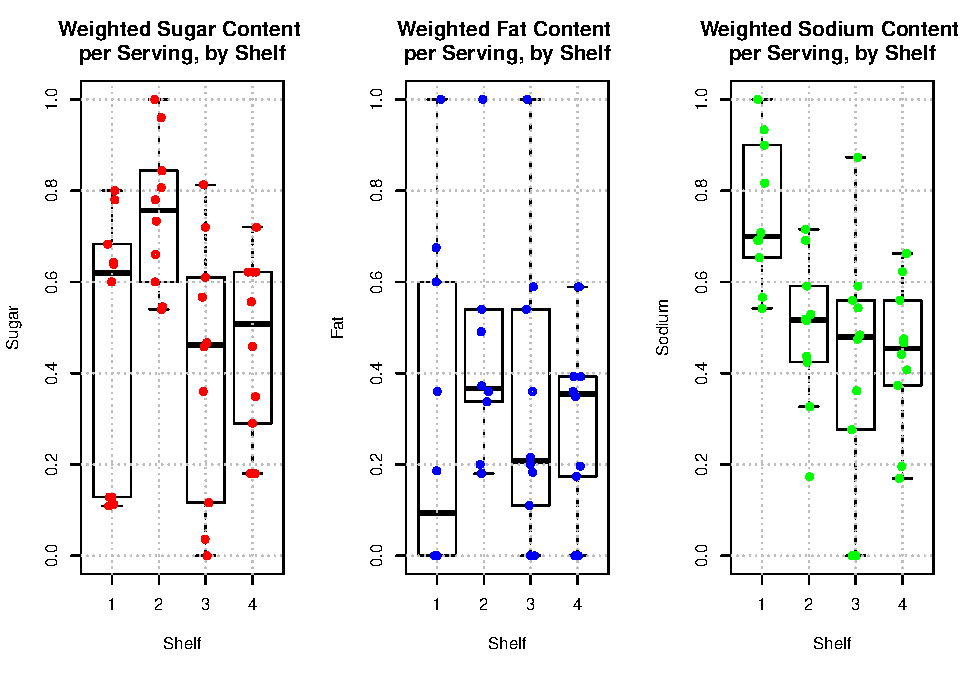
\includegraphics{HeatherFeinstein_DavidHarding_CharlotteSwavola.Rmd_files/figure-latex/unnamed-chunk-3-1.pdf}

\begin{Shaded}
\begin{Highlighting}[]
\KeywordTok{par}\NormalTok{(}\DataTypeTok{mar=}\KeywordTok{c}\NormalTok{(}\DecValTok{2}\NormalTok{, }\DecValTok{1}\NormalTok{, }\DecValTok{2}\NormalTok{, }\DecValTok{5}\NormalTok{),}\DataTypeTok{xpd =} \OtherTok{TRUE}\NormalTok{)}
\NormalTok{shelf.colors<-}\KeywordTok{ifelse}\NormalTok{(}\DataTypeTok{test =}\NormalTok{ cereal2}\OperatorTok{$}\NormalTok{Shelf}\OperatorTok{==}\StringTok{"1"}\NormalTok{, }\DataTypeTok{yes =} \StringTok{"black"}\NormalTok{, }
                    \DataTypeTok{no =} \KeywordTok{ifelse}\NormalTok{(}\DataTypeTok{test =}\NormalTok{ cereal2}\OperatorTok{$}\NormalTok{Shelf}\OperatorTok{==}\StringTok{"2"}\NormalTok{, }\DataTypeTok{yes =} \StringTok{"blue"}\NormalTok{, }\DataTypeTok{no =} \KeywordTok{ifelse}\NormalTok{(}\DataTypeTok{test =}\NormalTok{ cereal2}\OperatorTok{$}\NormalTok{Shelf}\OperatorTok{==}\StringTok{"3"}\NormalTok{, }\DataTypeTok{yes =} \StringTok{"green"}\NormalTok{, }\DataTypeTok{no =} \StringTok{"red"}\NormalTok{)))}
\KeywordTok{parcoord}\NormalTok{(}\DataTypeTok{x =}\NormalTok{ cereal2[, }\KeywordTok{c}\NormalTok{(}\DecValTok{2}\NormalTok{,}\DecValTok{3}\NormalTok{,}\DecValTok{4}\NormalTok{)], }\DataTypeTok{col =}\NormalTok{ shelf.colors, }\DataTypeTok{var.label =} \OtherTok{TRUE}\NormalTok{)}
\KeywordTok{title}\NormalTok{(}\DataTypeTok{main=}\StringTok{"Weighted Component Content by Shelf"}\NormalTok{)}
\KeywordTok{legend}\NormalTok{(}\DecValTok{3}\NormalTok{,}\FloatTok{0.5}\NormalTok{, }\DataTypeTok{legend =} \KeywordTok{c}\NormalTok{(}\StringTok{"Shelf 4"}\NormalTok{, }\StringTok{"Shelf 3"}\NormalTok{, }\StringTok{"Shelf 2"}\NormalTok{, }\StringTok{"Shelf 1"}\NormalTok{), }\DataTypeTok{lty =} \StringTok{"solid"}\NormalTok{,}
      \DataTypeTok{col=}\KeywordTok{c}\NormalTok{(}\StringTok{"red"}\NormalTok{, }\StringTok{"green"}\NormalTok{, }\StringTok{"blue"}\NormalTok{, }\StringTok{"black"}\NormalTok{), }\DataTypeTok{bty =} \StringTok{'n'}\NormalTok{)                   }
\end{Highlighting}
\end{Shaded}

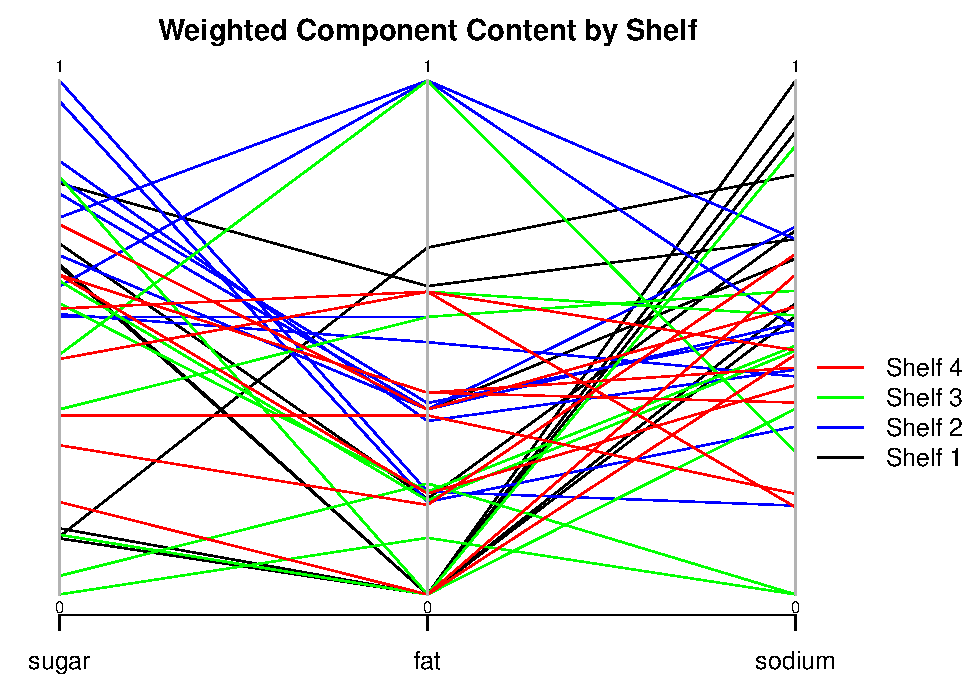
\includegraphics{HeatherFeinstein_DavidHarding_CharlotteSwavola.Rmd_files/figure-latex/unnamed-chunk-4-1.pdf}

\begin{enumerate}
\def\labelenumi{\alph{enumi}.}
\setcounter{enumi}{1}
\tightlist
\item
  (cont'd) Discuss if possible content differences exist among the
  shelves.\\
\end{enumerate}

\begin{itemize}
\tightlist
\item
  Shelf 1 has a higher, narrow sodium distribution relative to the wide
  distributions of other components and the sodium distribution - for
  other shelves.\\
\item
  Shelf 2 has a higher, narrow distribution for sugar content, and hits
  the maximum fat content (though not for all samples).\\
\item
  Shelf 3 maintains a wide distribution across all three components. It
  has the samples with the lowest sugar, fat, and sodium content.
\item
  Shelf 4 has wide distributions for all components that are generally
  lower than the component distributions of other shelves. \newpage
\end{itemize}

\begin{enumerate}
\def\labelenumi{\alph{enumi}.}
\setcounter{enumi}{2}
\tightlist
\item
  The response has values of \(1, 2, 3,\) and \(4\). Under what setting
  would it be desirable to take into account ordinality. Do you think
  that this setting occurs here?
\end{enumerate}

Ordinality could be considered for visibiility by a specific audience.
For example, if you were examining kids' cereal specifically, the
shelves would likely have the levels 2,1,3,4, for ordinality, as they
are the most likely to be seen in that order by that specific audience.
For fancy organic, perhaps 3,4,2,1- which corresponds to the eye levels
of (most) adults. In this case, we haven't specified a cereal type or a
particular audience to target, so an ordinality setting is not relevant.

\begin{enumerate}
\def\labelenumi{\alph{enumi}.}
\setcounter{enumi}{3}
\tightlist
\item
  Estimate a \textbf{multinomial regression model with linear forms of
  the sugar, fat, and sodium variables}. Perform \textbf{LRTs} to
  examine the importance of each explanatory variable.
\end{enumerate}

\begin{Shaded}
\begin{Highlighting}[]
\CommentTok{#Estimate model}
\NormalTok{mod.fit<-}\KeywordTok{multinom}\NormalTok{(}\DataTypeTok{formula =}\NormalTok{ Shelf }\OperatorTok{~}\StringTok{ }\NormalTok{sugar }\OperatorTok{+}\StringTok{ }\NormalTok{fat }\OperatorTok{+}\StringTok{ }\NormalTok{sodium, }\DataTypeTok{data=}\NormalTok{cereal2)}
\end{Highlighting}
\end{Shaded}

\begin{verbatim}
## # weights:  20 (12 variable)
## initial  value 55.451774 
## iter  10 value 37.329384
## iter  20 value 33.775257
## iter  30 value 33.608495
## iter  40 value 33.596631
## iter  50 value 33.595909
## iter  60 value 33.595564
## iter  70 value 33.595277
## iter  80 value 33.595147
## final  value 33.595139 
## converged
\end{verbatim}

\begin{Shaded}
\begin{Highlighting}[]
\KeywordTok{summary}\NormalTok{(mod.fit)}
\end{Highlighting}
\end{Shaded}

\begin{verbatim}
## Call:
## multinom(formula = Shelf ~ sugar + fat + sodium, data = cereal2)
## 
## Coefficients:
##   (Intercept)      sugar        fat    sodium
## 2    6.900708   2.693071  4.0647092 -17.49373
## 3   21.680680 -12.216442 -0.5571273 -24.97850
## 4   21.288343 -11.393710 -0.8701180 -24.67385
## 
## Std. Errors:
##   (Intercept)    sugar      fat   sodium
## 2    6.487408 5.051689 2.307250 7.097098
## 3    7.450885 4.887954 2.414963 8.080261
## 4    7.435125 4.871338 2.405710 8.062295
## 
## Residual Deviance: 67.19028 
## AIC: 91.19028
\end{verbatim}

\begin{Shaded}
\begin{Highlighting}[]
\CommentTok{# LRT for sugar_g:}
\NormalTok{mod.fit.Ho_sugar<-}\KeywordTok{multinom}\NormalTok{(}\DataTypeTok{formula =}\NormalTok{ Shelf }\OperatorTok{~}\StringTok{ }\NormalTok{fat }\OperatorTok{+}\StringTok{ }\NormalTok{sodium, }\DataTypeTok{data=}\NormalTok{cereal2, }\DataTypeTok{trace=}\OtherTok{FALSE}\NormalTok{)}
\KeywordTok{anova}\NormalTok{(mod.fit.Ho_sugar, mod.fit)  }
\end{Highlighting}
\end{Shaded}

\begin{verbatim}
## Likelihood ratio tests of Multinomial Models
## 
## Response: Shelf
##                  Model Resid. df Resid. Dev   Test    Df LR stat.
## 1         fat + sodium       111   89.95511                      
## 2 sugar + fat + sodium       108   67.19028 1 vs 2     3 22.76484
##        Pr(Chi)
## 1             
## 2 4.520699e-05
\end{verbatim}

The p-value for the likelihood ratio test is less than 0.05, therefore
we can reject the null hypothesis for sugar, concluding that sugar is
significant to the model.

\begin{Shaded}
\begin{Highlighting}[]
\CommentTok{# LRT for fat_g:}
\NormalTok{mod.fit.Ho_fat<-}\KeywordTok{multinom}\NormalTok{(}\DataTypeTok{formula =}\NormalTok{ Shelf }\OperatorTok{~}\StringTok{ }\NormalTok{sugar }\OperatorTok{+}\StringTok{ }\NormalTok{sodium, }\DataTypeTok{data=}\NormalTok{cereal2, }\DataTypeTok{trace=}\OtherTok{FALSE}\NormalTok{)}
\KeywordTok{anova}\NormalTok{(mod.fit.Ho_fat, mod.fit)   }
\end{Highlighting}
\end{Shaded}

\begin{verbatim}
## Likelihood ratio tests of Multinomial Models
## 
## Response: Shelf
##                  Model Resid. df Resid. Dev   Test    Df LR stat.
## 1       sugar + sodium       111   72.47384                      
## 2 sugar + fat + sodium       108   67.19028 1 vs 2     3  5.28356
##     Pr(Chi)
## 1          
## 2 0.1521727
\end{verbatim}

We cannot reject the null hypothesis that fat is not significant to the
model.

\begin{Shaded}
\begin{Highlighting}[]
\CommentTok{# LRT for sodium_mg:}
\NormalTok{mod.fit.Ho_sodium<-}\KeywordTok{multinom}\NormalTok{(}\DataTypeTok{formula =}\NormalTok{ Shelf }\OperatorTok{~}\StringTok{ }\NormalTok{sugar }\OperatorTok{+}\StringTok{ }\NormalTok{fat, }\DataTypeTok{data=}\NormalTok{cereal2, }\DataTypeTok{trace=}\OtherTok{FALSE}\NormalTok{)}
\KeywordTok{anova}\NormalTok{(mod.fit.Ho_sodium, mod.fit)   }
\end{Highlighting}
\end{Shaded}

\begin{verbatim}
## Likelihood ratio tests of Multinomial Models
## 
## Response: Shelf
##                  Model Resid. df Resid. Dev   Test    Df LR stat.
## 1          sugar + fat       111   93.81001                      
## 2 sugar + fat + sodium       108   67.19028 1 vs 2     3 26.61974
##        Pr(Chi)
## 1             
## 2 7.073281e-06
\end{verbatim}

For sodium, the p-value is less than 0.05. We can reject the null
hypothesis and conclude that sodium is significant to the model

\newpage

\begin{enumerate}
\def\labelenumi{\alph{enumi}.}
\setcounter{enumi}{4}
\tightlist
\item
  Show that there are no significant interactions among the explanatory
  variables (including an interaction among all three variables).
\end{enumerate}

\begin{Shaded}
\begin{Highlighting}[]
\CommentTok{# LRT for sugar*sodium interaction term:}
\NormalTok{mod.fit.Ho_sugar_sodium <-}\StringTok{ }\KeywordTok{multinom}\NormalTok{(}\DataTypeTok{formula =}\NormalTok{ Shelf }\OperatorTok{~}\StringTok{ }\NormalTok{sugar }\OperatorTok{+}\StringTok{ }\NormalTok{fat }\OperatorTok{+}\StringTok{ }\NormalTok{sodium }\OperatorTok{+}\StringTok{ }\NormalTok{sugar}\OperatorTok{:}\NormalTok{sodium, }\DataTypeTok{data=}\NormalTok{cereal2, }\DataTypeTok{maxit=}\DecValTok{200}\NormalTok{, }\DataTypeTok{trace=}\OtherTok{FALSE}\NormalTok{)}
\KeywordTok{anova}\NormalTok{(mod.fit.Ho_sugar_sodium, mod.fit)   }
\end{Highlighting}
\end{Shaded}

\begin{verbatim}
## Likelihood ratio tests of Multinomial Models
## 
## Response: Shelf
##                                 Model Resid. df Resid. Dev   Test    Df
## 1                sugar + fat + sodium       108   67.19028             
## 2 sugar + fat + sodium + sugar:sodium       105   64.83988 1 vs 2     3
##   LR stat.  Pr(Chi)
## 1                  
## 2 2.350397 0.502935
\end{verbatim}

\begin{Shaded}
\begin{Highlighting}[]
\CommentTok{# LRT for sugar*fat interaction term:}
\NormalTok{mod.fit.Ho_sugar_fat <-}\StringTok{ }\KeywordTok{multinom}\NormalTok{(}\DataTypeTok{formula =}\NormalTok{ Shelf }\OperatorTok{~}\StringTok{ }\NormalTok{sugar }\OperatorTok{+}\StringTok{ }\NormalTok{fat }\OperatorTok{+}\StringTok{ }\NormalTok{sodium }\OperatorTok{+}\StringTok{ }\NormalTok{sugar}\OperatorTok{:}\NormalTok{fat, }\DataTypeTok{data=}\NormalTok{cereal2, }\DataTypeTok{maxit=}\DecValTok{200}\NormalTok{, }\DataTypeTok{trace=}\OtherTok{FALSE}\NormalTok{)}
\KeywordTok{anova}\NormalTok{(mod.fit.Ho_sugar_fat, mod.fit)  }
\end{Highlighting}
\end{Shaded}

\begin{verbatim}
## Likelihood ratio tests of Multinomial Models
## 
## Response: Shelf
##                              Model Resid. df Resid. Dev   Test    Df
## 1             sugar + fat + sodium       108   67.19028             
## 2 sugar + fat + sodium + sugar:fat       105   61.82907 1 vs 2     3
##   LR stat.   Pr(Chi)
## 1                   
## 2  5.36121 0.1471795
\end{verbatim}

\begin{Shaded}
\begin{Highlighting}[]
\CommentTok{# LRT for fat*sodium interaction term:}
\NormalTok{mod.fit.Ho_fat_sodium <-}\StringTok{ }\KeywordTok{multinom}\NormalTok{(}\DataTypeTok{formula =}\NormalTok{ Shelf }\OperatorTok{~}\StringTok{ }\NormalTok{sugar }\OperatorTok{+}\StringTok{ }\NormalTok{fat }\OperatorTok{+}\StringTok{ }\NormalTok{sodium }\OperatorTok{+}\StringTok{ }\NormalTok{sugar}\OperatorTok{:}\NormalTok{sodium, }\DataTypeTok{data=}\NormalTok{cereal2, }\DataTypeTok{maxit=}\DecValTok{200}\NormalTok{, }\DataTypeTok{trace=}\OtherTok{FALSE}\NormalTok{)}
\KeywordTok{anova}\NormalTok{(mod.fit.Ho_fat_sodium, mod.fit)  }
\end{Highlighting}
\end{Shaded}

\begin{verbatim}
## Likelihood ratio tests of Multinomial Models
## 
## Response: Shelf
##                                 Model Resid. df Resid. Dev   Test    Df
## 1                sugar + fat + sodium       108   67.19028             
## 2 sugar + fat + sodium + sugar:sodium       105   64.83988 1 vs 2     3
##   LR stat.  Pr(Chi)
## 1                  
## 2 2.350397 0.502935
\end{verbatim}

\begin{Shaded}
\begin{Highlighting}[]
\CommentTok{# LRT for sugar*fat*sodium interaction term:}
\NormalTok{mod.fit.Ho_sugar_fat_sodium <-}\StringTok{ }\KeywordTok{multinom}\NormalTok{(}\DataTypeTok{formula =}\NormalTok{ Shelf }\OperatorTok{~}\StringTok{ }\NormalTok{sugar }\OperatorTok{+}\StringTok{ }\NormalTok{fat }\OperatorTok{+}\StringTok{ }\NormalTok{sodium }\OperatorTok{+}\StringTok{ }\NormalTok{sugar}\OperatorTok{:}\NormalTok{fat}\OperatorTok{:}\NormalTok{sodium, }\DataTypeTok{data=}\NormalTok{cereal2, }\DataTypeTok{maxit=}\DecValTok{200}\NormalTok{, }\DataTypeTok{trace=}\OtherTok{FALSE}\NormalTok{)}
\KeywordTok{anova}\NormalTok{(mod.fit.Ho_sugar_fat_sodium, mod.fit)  }
\end{Highlighting}
\end{Shaded}

\begin{verbatim}
## Likelihood ratio tests of Multinomial Models
## 
## Response: Shelf
##                                     Model Resid. df Resid. Dev   Test
## 1                    sugar + fat + sodium       108   67.19028       
## 2 sugar + fat + sodium + sugar:fat:sodium       105   65.04570 1 vs 2
##      Df LR stat.   Pr(Chi)
## 1                         
## 2     3  2.14458 0.5429468
\end{verbatim}

We cannot reject any of the null hypotheses for the possible interaction
coefficients. These interaction coefficients are not significant to the
model.

\begin{enumerate}
\def\labelenumi{\alph{enumi}.}
\setcounter{enumi}{5}
\tightlist
\item
  Kellogg's Apple Jacks (\url{http://www.applejacks.com}) is a cereal
  marketed toward children. For a serving size of \(28\) grams, its
  sugar content is \(12\) grams, fat content is \(0.5\) grams, and
  sodium content is \(130\) milligrams. Estimate the shelf probabilities
  for Apple Jacks.
\end{enumerate}

\begin{Shaded}
\begin{Highlighting}[]
\CommentTok{# Data for Apple Jacks standardized}
\NormalTok{stand01.spec <-}\StringTok{ }\ControlFlowTok{function}\NormalTok{(w,x) \{(w }\OperatorTok{-}\StringTok{ }\KeywordTok{min}\NormalTok{(x)) }\OperatorTok{/}\NormalTok{( }\KeywordTok{max}\NormalTok{(x) }\OperatorTok{-}\StringTok{ }\KeywordTok{min}\NormalTok{(x))\} }
\NormalTok{newdata <-}\StringTok{ }\KeywordTok{data.frame}\NormalTok{(}\DataTypeTok{sugar =} \KeywordTok{stand01.spec}\NormalTok{(}\DataTypeTok{w =} \DecValTok{12}\OperatorTok{/}\DecValTok{28}\NormalTok{, }\DataTypeTok{x =}\NormalTok{ cereal}\OperatorTok{$}\NormalTok{sugar_g}\OperatorTok{/}\NormalTok{cereal}\OperatorTok{$}\NormalTok{size_g), }
                      \DataTypeTok{fat =} \KeywordTok{stand01.spec}\NormalTok{(}\DataTypeTok{w =} \FloatTok{0.5}\OperatorTok{/}\DecValTok{28}\NormalTok{, }\DataTypeTok{x =}\NormalTok{ cereal}\OperatorTok{$}\NormalTok{fat_g}\OperatorTok{/}\NormalTok{cereal}\OperatorTok{$}\NormalTok{size_g), }
                      \DataTypeTok{sodium =} \KeywordTok{stand01.spec}\NormalTok{(}\DataTypeTok{w =} \DecValTok{130}\OperatorTok{/}\DecValTok{28}\NormalTok{, }\DataTypeTok{x =}\NormalTok{ cereal}\OperatorTok{$}\NormalTok{sodium_mg}\OperatorTok{/}\NormalTok{cereal}\OperatorTok{$}\NormalTok{size_g))}
\NormalTok{newdata}
\end{Highlighting}
\end{Shaded}

\begin{verbatim}
##       sugar       fat    sodium
## 1 0.7714286 0.1928571 0.4333333
\end{verbatim}

\begin{Shaded}
\begin{Highlighting}[]
\CommentTok{# pi^}
\NormalTok{pi.hat<-}\KeywordTok{predict}\NormalTok{(}\DataTypeTok{object =}\NormalTok{ mod.fit, }\DataTypeTok{newdata =}\NormalTok{ newdata, }\DataTypeTok{type =} \StringTok{"probs"}\NormalTok{)}
\KeywordTok{round}\NormalTok{(pi.hat, }\DecValTok{2}\NormalTok{)}
\end{Highlighting}
\end{Shaded}

\begin{verbatim}
##    1    2    3    4 
## 0.05 0.47 0.20 0.27
\end{verbatim}

\begin{enumerate}
\def\labelenumi{\alph{enumi}.}
\setcounter{enumi}{6}
\tightlist
\item
  Construct a plot similar to \textbf{Figure 3.3} where the estimated
  probability for a shelf is on the \emph{y-axis} and the sugar content
  is on the \emph{x-axis}. Use the mean overall fat and sodium content
  as the corresponding variable values in the model. Interpret the plot
  with respect to sugar content.
\end{enumerate}

\begin{Shaded}
\begin{Highlighting}[]
\KeywordTok{curve}\NormalTok{(}\DataTypeTok{expr =} \KeywordTok{predict}\NormalTok{(}\DataTypeTok{object =}\NormalTok{ mod.fit, }\DataTypeTok{newdata =} \KeywordTok{data.frame}\NormalTok{(}\DataTypeTok{sugar =}\NormalTok{ x,}
      \DataTypeTok{fat =} \KeywordTok{mean}\NormalTok{(cereal2}\OperatorTok{$}\NormalTok{fat), }\DataTypeTok{sodium =} \KeywordTok{mean}\NormalTok{(cereal2}\OperatorTok{$}\NormalTok{sodium)), }\DataTypeTok{type =} \StringTok{"probs"}\NormalTok{)[,}\DecValTok{1}\NormalTok{], }
      \DataTypeTok{main=} \KeywordTok{expression}\NormalTok{(Shelf}\OperatorTok{~}\KeywordTok{hat}\NormalTok{(pi)}\OperatorTok{~}\StringTok{"vs Sugar content"}\NormalTok{),}
      \DataTypeTok{ylab =} \KeywordTok{expression}\NormalTok{(Shelf}\OperatorTok{~}\KeywordTok{hat}\NormalTok{(pi)), }\DataTypeTok{xlab =} \StringTok{"Sugar"}\NormalTok{, }\DataTypeTok{xlim =} \KeywordTok{c}\NormalTok{(}\KeywordTok{min}\NormalTok{(cereal2}\OperatorTok{$}\NormalTok{sugar), }\KeywordTok{max}\NormalTok{(cereal2}\OperatorTok{$}\NormalTok{sugar)), }
      \DataTypeTok{ylim =} \KeywordTok{c}\NormalTok{(}\DecValTok{0}\NormalTok{,}\DecValTok{1}\NormalTok{), }\DataTypeTok{col =} \StringTok{"black"}\NormalTok{, }\DataTypeTok{lty =} \StringTok{"solid"}\NormalTok{, }\DataTypeTok{lwd =} \DecValTok{2}\NormalTok{, }\DataTypeTok{n =} \DecValTok{1000}\NormalTok{,}
      \DataTypeTok{panel.first =} \KeywordTok{grid}\NormalTok{(}\DataTypeTok{col =} \StringTok{"gray"}\NormalTok{, }\DataTypeTok{lty =} \StringTok{"dotted"}\NormalTok{))}

\KeywordTok{curve}\NormalTok{(}\DataTypeTok{expr =} \KeywordTok{predict}\NormalTok{(}\DataTypeTok{object =}\NormalTok{ mod.fit, }\DataTypeTok{newdata =} \KeywordTok{data.frame}\NormalTok{(}\DataTypeTok{sugar =}\NormalTok{ x,}
      \DataTypeTok{fat =} \KeywordTok{mean}\NormalTok{(cereal2}\OperatorTok{$}\NormalTok{fat), }\DataTypeTok{sodium =} \KeywordTok{mean}\NormalTok{(cereal2}\OperatorTok{$}\NormalTok{sodium)), }\DataTypeTok{type =} \StringTok{"probs"}\NormalTok{)[,}\DecValTok{2}\NormalTok{], }
      \DataTypeTok{col =} \StringTok{"blue"}\NormalTok{, }\DataTypeTok{lty =} \StringTok{"solid"}\NormalTok{, }\DataTypeTok{lwd =} \DecValTok{2}\NormalTok{, }\DataTypeTok{n =} \DecValTok{1000}\NormalTok{,}
      \DataTypeTok{add =} \OtherTok{TRUE}\NormalTok{, }\DataTypeTok{panel.first =} \KeywordTok{grid}\NormalTok{(}\DataTypeTok{col =} \StringTok{"gray"}\NormalTok{, }\DataTypeTok{lty =} \StringTok{"dotted"}\NormalTok{))}

\KeywordTok{curve}\NormalTok{(}\DataTypeTok{expr =} \KeywordTok{predict}\NormalTok{(}\DataTypeTok{object =}\NormalTok{ mod.fit, }\DataTypeTok{newdata =} \KeywordTok{data.frame}\NormalTok{(}\DataTypeTok{sugar =}\NormalTok{ x,}
      \DataTypeTok{fat =} \KeywordTok{mean}\NormalTok{(cereal2}\OperatorTok{$}\NormalTok{fat), }\DataTypeTok{sodium =} \KeywordTok{mean}\NormalTok{(cereal2}\OperatorTok{$}\NormalTok{sodium)), }\DataTypeTok{type =} \StringTok{"probs"}\NormalTok{)[,}\DecValTok{3}\NormalTok{], }
      \DataTypeTok{col =} \StringTok{"green"}\NormalTok{, }\DataTypeTok{lty =} \StringTok{"solid"}\NormalTok{, }\DataTypeTok{lwd =} \DecValTok{2}\NormalTok{, }\DataTypeTok{n =} \DecValTok{1000}\NormalTok{,}
      \DataTypeTok{add =} \OtherTok{TRUE}\NormalTok{, }\DataTypeTok{panel.first =} \KeywordTok{grid}\NormalTok{(}\DataTypeTok{col =} \StringTok{"gray"}\NormalTok{, }\DataTypeTok{lty =} \StringTok{"dotted"}\NormalTok{))}

\KeywordTok{curve}\NormalTok{(}\DataTypeTok{expr =} \KeywordTok{predict}\NormalTok{(}\DataTypeTok{object =}\NormalTok{ mod.fit, }\DataTypeTok{newdata =} \KeywordTok{data.frame}\NormalTok{(}\DataTypeTok{sugar =}\NormalTok{ x,}
      \DataTypeTok{fat =} \KeywordTok{mean}\NormalTok{(cereal2}\OperatorTok{$}\NormalTok{fat), }\DataTypeTok{sodium =} \KeywordTok{mean}\NormalTok{(cereal2}\OperatorTok{$}\NormalTok{sodium)), }\DataTypeTok{type =} \StringTok{"probs"}\NormalTok{)[,}\DecValTok{4}\NormalTok{], }
      \DataTypeTok{col =} \StringTok{"red"}\NormalTok{, }\DataTypeTok{lty =} \StringTok{"solid"}\NormalTok{, }\DataTypeTok{lwd =} \DecValTok{2}\NormalTok{, }\DataTypeTok{n =} \DecValTok{1000}\NormalTok{,}
      \DataTypeTok{add =} \OtherTok{TRUE}\NormalTok{, }\DataTypeTok{panel.first =} \KeywordTok{grid}\NormalTok{(}\DataTypeTok{col =} \StringTok{"gray"}\NormalTok{, }\DataTypeTok{lty =} \StringTok{"dotted"}\NormalTok{))}

\KeywordTok{legend}\NormalTok{(}\DataTypeTok{x=}\FloatTok{0.2}\NormalTok{,}\DataTypeTok{y=}\DecValTok{1}\NormalTok{, }\DataTypeTok{legend=}\KeywordTok{c}\NormalTok{(}\StringTok{"Shelf 4"}\NormalTok{,}\StringTok{"Shelf 3"}\NormalTok{,}\StringTok{"Shelf 2"}\NormalTok{, }\StringTok{"Shelf 1"}\NormalTok{), }\DataTypeTok{lty=}\KeywordTok{c}\NormalTok{(}\StringTok{"solid"}\NormalTok{), }\DataTypeTok{col=}\KeywordTok{c}\NormalTok{(}\StringTok{"red"}\NormalTok{,}\StringTok{"green"}\NormalTok{, }\StringTok{"blue"}\NormalTok{, }\StringTok{"black"}\NormalTok{), }\DataTypeTok{bty=}\StringTok{"n"}\NormalTok{, }\DataTypeTok{lwd =} \KeywordTok{c}\NormalTok{(}\DecValTok{2}\NormalTok{,}\DecValTok{2}\NormalTok{,}\DecValTok{2}\NormalTok{))}
\end{Highlighting}
\end{Shaded}

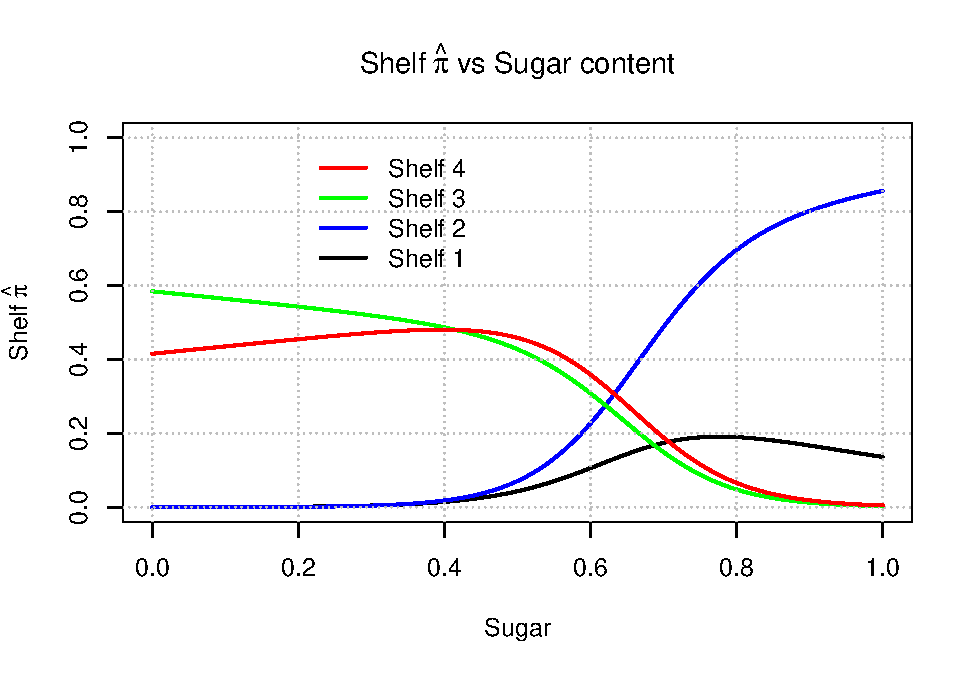
\includegraphics{HeatherFeinstein_DavidHarding_CharlotteSwavola.Rmd_files/figure-latex/unnamed-chunk-11-1.pdf}

\begin{Shaded}
\begin{Highlighting}[]
\KeywordTok{par}\NormalTok{(}\DataTypeTok{mfrow=}\KeywordTok{c}\NormalTok{(}\DecValTok{1}\NormalTok{,}\DecValTok{2}\NormalTok{))}
\KeywordTok{curve}\NormalTok{(}\DataTypeTok{expr =} \KeywordTok{predict}\NormalTok{(}\DataTypeTok{object =}\NormalTok{ mod.fit, }\DataTypeTok{newdata =} \KeywordTok{data.frame}\NormalTok{(}\DataTypeTok{sugar =} \KeywordTok{mean}\NormalTok{(cereal2}\OperatorTok{$}\NormalTok{sugar),}
      \DataTypeTok{fat =}\NormalTok{x, }\DataTypeTok{sodium =} \KeywordTok{mean}\NormalTok{(cereal2}\OperatorTok{$}\NormalTok{sodium)), }\DataTypeTok{type =} \StringTok{"probs"}\NormalTok{)[,}\DecValTok{1}\NormalTok{],}
      \DataTypeTok{main=} \KeywordTok{expression}\NormalTok{(Shelf}\OperatorTok{~}\KeywordTok{hat}\NormalTok{(pi)}\OperatorTok{~}\StringTok{"vs Fat"}\NormalTok{),}
      \DataTypeTok{ylab =} \KeywordTok{expression}\NormalTok{(Shelf}\OperatorTok{~}\KeywordTok{hat}\NormalTok{(pi)), }\DataTypeTok{xlab =} \StringTok{"Fat"}\NormalTok{, }\DataTypeTok{xlim =} \KeywordTok{c}\NormalTok{(}\KeywordTok{min}\NormalTok{(cereal2}\OperatorTok{$}\NormalTok{fat), }\KeywordTok{max}\NormalTok{(cereal2}\OperatorTok{$}\NormalTok{fat)), }
      \DataTypeTok{ylim =} \KeywordTok{c}\NormalTok{(}\DecValTok{0}\NormalTok{,}\DecValTok{1}\NormalTok{), }\DataTypeTok{col =} \StringTok{"black"}\NormalTok{, }\DataTypeTok{lty =} \StringTok{"solid"}\NormalTok{, }\DataTypeTok{lwd =} \DecValTok{2}\NormalTok{, }\DataTypeTok{n =} \DecValTok{1000}\NormalTok{,}
      \DataTypeTok{panel.first =} \KeywordTok{grid}\NormalTok{(}\DataTypeTok{col =} \StringTok{"gray"}\NormalTok{, }\DataTypeTok{lty =} \StringTok{"dotted"}\NormalTok{))}

\KeywordTok{curve}\NormalTok{(}\DataTypeTok{expr =} \KeywordTok{predict}\NormalTok{(}\DataTypeTok{object =}\NormalTok{ mod.fit, }\DataTypeTok{newdata =} \KeywordTok{data.frame}\NormalTok{(}\DataTypeTok{sugar =} \KeywordTok{mean}\NormalTok{(cereal2}\OperatorTok{$}\NormalTok{sugar),}
      \DataTypeTok{fat =}\NormalTok{x, }\DataTypeTok{sodium =} \KeywordTok{mean}\NormalTok{(cereal2}\OperatorTok{$}\NormalTok{sodium)), }\DataTypeTok{type =} \StringTok{"probs"}\NormalTok{)[,}\DecValTok{2}\NormalTok{], }
      \DataTypeTok{col =} \StringTok{"blue"}\NormalTok{, }\DataTypeTok{lty =} \StringTok{"solid"}\NormalTok{, }\DataTypeTok{lwd =} \DecValTok{2}\NormalTok{, }\DataTypeTok{n =} \DecValTok{1000}\NormalTok{,}
      \DataTypeTok{add =} \OtherTok{TRUE}\NormalTok{, }\DataTypeTok{panel.first =} \KeywordTok{grid}\NormalTok{(}\DataTypeTok{col =} \StringTok{"gray"}\NormalTok{, }\DataTypeTok{lty =} \StringTok{"dotted"}\NormalTok{))}

\KeywordTok{curve}\NormalTok{(}\DataTypeTok{expr =} \KeywordTok{predict}\NormalTok{(}\DataTypeTok{object =}\NormalTok{ mod.fit, }\DataTypeTok{newdata =} \KeywordTok{data.frame}\NormalTok{(}\DataTypeTok{sugar =} \KeywordTok{mean}\NormalTok{(cereal2}\OperatorTok{$}\NormalTok{sugar),}
      \DataTypeTok{fat =}\NormalTok{x, }\DataTypeTok{sodium =} \KeywordTok{mean}\NormalTok{(cereal2}\OperatorTok{$}\NormalTok{sodium)), }\DataTypeTok{type =} \StringTok{"probs"}\NormalTok{)[,}\DecValTok{3}\NormalTok{], }
      \DataTypeTok{col =} \StringTok{"green"}\NormalTok{, }\DataTypeTok{lty =} \StringTok{"solid"}\NormalTok{, }\DataTypeTok{lwd =} \DecValTok{2}\NormalTok{, }\DataTypeTok{n =} \DecValTok{1000}\NormalTok{,}
      \DataTypeTok{add =} \OtherTok{TRUE}\NormalTok{, }\DataTypeTok{panel.first =} \KeywordTok{grid}\NormalTok{(}\DataTypeTok{col =} \StringTok{"gray"}\NormalTok{, }\DataTypeTok{lty =} \StringTok{"dotted"}\NormalTok{))}

\KeywordTok{curve}\NormalTok{(}\DataTypeTok{expr =} \KeywordTok{predict}\NormalTok{(}\DataTypeTok{object =}\NormalTok{ mod.fit, }\DataTypeTok{newdata =} \KeywordTok{data.frame}\NormalTok{(}\DataTypeTok{sugar =} \KeywordTok{mean}\NormalTok{(cereal2}\OperatorTok{$}\NormalTok{sugar),}
      \DataTypeTok{fat =}\NormalTok{x, }\DataTypeTok{sodium =} \KeywordTok{mean}\NormalTok{(cereal2}\OperatorTok{$}\NormalTok{sodium)), }\DataTypeTok{type =} \StringTok{"probs"}\NormalTok{)[,}\DecValTok{4}\NormalTok{], }
      \DataTypeTok{col =} \StringTok{"red"}\NormalTok{, }\DataTypeTok{lty =} \StringTok{"solid"}\NormalTok{, }\DataTypeTok{lwd =} \DecValTok{2}\NormalTok{, }\DataTypeTok{n =} \DecValTok{1000}\NormalTok{,}
      \DataTypeTok{add =} \OtherTok{TRUE}\NormalTok{, }\DataTypeTok{panel.first =} \KeywordTok{grid}\NormalTok{(}\DataTypeTok{col =} \StringTok{"gray"}\NormalTok{, }\DataTypeTok{lty =} \StringTok{"dotted"}\NormalTok{))}

\KeywordTok{legend}\NormalTok{(}\DataTypeTok{x=}\DecValTok{0}\NormalTok{,}\DataTypeTok{y=}\DecValTok{1}\NormalTok{, }\DataTypeTok{legend=}\KeywordTok{c}\NormalTok{(}\StringTok{"Shelf 4"}\NormalTok{,}\StringTok{"Shelf 3"}\NormalTok{,}\StringTok{"Shelf 2"}\NormalTok{, }\StringTok{"Shelf 1"}\NormalTok{), }\DataTypeTok{lty=}\KeywordTok{c}\NormalTok{(}\StringTok{"solid"}\NormalTok{), }\DataTypeTok{col=}\KeywordTok{c}\NormalTok{(}\StringTok{"red"}\NormalTok{,}\StringTok{"green"}\NormalTok{, }\StringTok{"blue"}\NormalTok{, }\StringTok{"black"}\NormalTok{), }\DataTypeTok{bty=}\StringTok{"n"}\NormalTok{, }\DataTypeTok{lwd =} \KeywordTok{c}\NormalTok{(}\DecValTok{2}\NormalTok{,}\DecValTok{2}\NormalTok{,}\DecValTok{2}\NormalTok{))}

\KeywordTok{curve}\NormalTok{(}\DataTypeTok{expr =} \KeywordTok{predict}\NormalTok{(}\DataTypeTok{object =}\NormalTok{ mod.fit, }\DataTypeTok{newdata =} \KeywordTok{data.frame}\NormalTok{(}\DataTypeTok{sugar =} \KeywordTok{mean}\NormalTok{(cereal2}\OperatorTok{$}\NormalTok{sugar),}
      \DataTypeTok{fat =} \KeywordTok{mean}\NormalTok{(cereal2}\OperatorTok{$}\NormalTok{fat), }\DataTypeTok{sodium =}\NormalTok{ x), }\DataTypeTok{type =} \StringTok{"probs"}\NormalTok{)[,}\DecValTok{1}\NormalTok{],}
      \DataTypeTok{main=} \KeywordTok{expression}\NormalTok{(Shelf}\OperatorTok{~}\KeywordTok{hat}\NormalTok{(pi)}\OperatorTok{~}\StringTok{"vs Sodium"}\NormalTok{),}
      \DataTypeTok{ylab =} \KeywordTok{expression}\NormalTok{(Shelf}\OperatorTok{~}\KeywordTok{hat}\NormalTok{(pi)), }\DataTypeTok{xlab =} \StringTok{"Sodium"}\NormalTok{, }\DataTypeTok{xlim =} \KeywordTok{c}\NormalTok{(}\KeywordTok{min}\NormalTok{(cereal2}\OperatorTok{$}\NormalTok{sodium), }\KeywordTok{max}\NormalTok{(cereal2}\OperatorTok{$}\NormalTok{sodium)), }
      \DataTypeTok{ylim =} \KeywordTok{c}\NormalTok{(}\DecValTok{0}\NormalTok{,}\DecValTok{1}\NormalTok{), }\DataTypeTok{col =} \StringTok{"black"}\NormalTok{, }\DataTypeTok{lty =} \StringTok{"solid"}\NormalTok{, }\DataTypeTok{lwd =} \DecValTok{2}\NormalTok{, }\DataTypeTok{n =} \DecValTok{1000}\NormalTok{,}
      \DataTypeTok{panel.first =} \KeywordTok{grid}\NormalTok{(}\DataTypeTok{col =} \StringTok{"gray"}\NormalTok{, }\DataTypeTok{lty =} \StringTok{"dotted"}\NormalTok{))}

\KeywordTok{curve}\NormalTok{(}\DataTypeTok{expr =} \KeywordTok{predict}\NormalTok{(}\DataTypeTok{object =}\NormalTok{ mod.fit, }\DataTypeTok{newdata =} \KeywordTok{data.frame}\NormalTok{(}\DataTypeTok{sugar =} \KeywordTok{mean}\NormalTok{(cereal2}\OperatorTok{$}\NormalTok{sugar),}
      \DataTypeTok{fat =} \KeywordTok{mean}\NormalTok{(cereal2}\OperatorTok{$}\NormalTok{fat), }\DataTypeTok{sodium =}\NormalTok{ x), }\DataTypeTok{type =} \StringTok{"probs"}\NormalTok{)[,}\DecValTok{2}\NormalTok{], }
      \DataTypeTok{col =} \StringTok{"blue"}\NormalTok{, }\DataTypeTok{lty =} \StringTok{"solid"}\NormalTok{, }\DataTypeTok{lwd =} \DecValTok{2}\NormalTok{, }\DataTypeTok{n =} \DecValTok{1000}\NormalTok{,}
      \DataTypeTok{add =} \OtherTok{TRUE}\NormalTok{, }\DataTypeTok{panel.first =} \KeywordTok{grid}\NormalTok{(}\DataTypeTok{col =} \StringTok{"gray"}\NormalTok{, }\DataTypeTok{lty =} \StringTok{"dotted"}\NormalTok{))}

\KeywordTok{curve}\NormalTok{(}\DataTypeTok{expr =} \KeywordTok{predict}\NormalTok{(}\DataTypeTok{object =}\NormalTok{ mod.fit, }\DataTypeTok{newdata =} \KeywordTok{data.frame}\NormalTok{(}\DataTypeTok{sugar =} \KeywordTok{mean}\NormalTok{(cereal2}\OperatorTok{$}\NormalTok{sugar),}
      \DataTypeTok{fat =} \KeywordTok{mean}\NormalTok{(cereal2}\OperatorTok{$}\NormalTok{fat), }\DataTypeTok{sodium =}\NormalTok{ x), }\DataTypeTok{type =} \StringTok{"probs"}\NormalTok{)[,}\DecValTok{3}\NormalTok{], }
      \DataTypeTok{col =} \StringTok{"green"}\NormalTok{, }\DataTypeTok{lty =} \StringTok{"solid"}\NormalTok{, }\DataTypeTok{lwd =} \DecValTok{2}\NormalTok{, }\DataTypeTok{n =} \DecValTok{1000}\NormalTok{,}
      \DataTypeTok{add =} \OtherTok{TRUE}\NormalTok{, }\DataTypeTok{panel.first =} \KeywordTok{grid}\NormalTok{(}\DataTypeTok{col =} \StringTok{"gray"}\NormalTok{, }\DataTypeTok{lty =} \StringTok{"dotted"}\NormalTok{))}

\KeywordTok{curve}\NormalTok{(}\DataTypeTok{expr =} \KeywordTok{predict}\NormalTok{(}\DataTypeTok{object =}\NormalTok{ mod.fit, }\DataTypeTok{newdata =} \KeywordTok{data.frame}\NormalTok{(}\DataTypeTok{sugar =} \KeywordTok{mean}\NormalTok{(cereal2}\OperatorTok{$}\NormalTok{sugar),}
      \DataTypeTok{fat =} \KeywordTok{mean}\NormalTok{(cereal2}\OperatorTok{$}\NormalTok{fat), }\DataTypeTok{sodium =}\NormalTok{ x), }\DataTypeTok{type =} \StringTok{"probs"}\NormalTok{)[,}\DecValTok{4}\NormalTok{], }
      \DataTypeTok{col =} \StringTok{"red"}\NormalTok{, }\DataTypeTok{lty =} \StringTok{"solid"}\NormalTok{, }\DataTypeTok{lwd =} \DecValTok{2}\NormalTok{, }\DataTypeTok{n =} \DecValTok{1000}\NormalTok{,}
      \DataTypeTok{add =} \OtherTok{TRUE}\NormalTok{, }\DataTypeTok{panel.first =} \KeywordTok{grid}\NormalTok{(}\DataTypeTok{col =} \StringTok{"gray"}\NormalTok{, }\DataTypeTok{lty =} \StringTok{"dotted"}\NormalTok{))}

\KeywordTok{legend}\NormalTok{(}\DataTypeTok{x=}\DecValTok{0}\NormalTok{,}\DataTypeTok{y=}\DecValTok{1}\NormalTok{, }\DataTypeTok{legend=}\KeywordTok{c}\NormalTok{(}\StringTok{"Shelf 4"}\NormalTok{,}\StringTok{"Shelf 3"}\NormalTok{,}\StringTok{"Shelf 2"}\NormalTok{, }\StringTok{"Shelf 1"}\NormalTok{), }\DataTypeTok{lty=}\KeywordTok{c}\NormalTok{(}\StringTok{"solid"}\NormalTok{), }\DataTypeTok{col=}\KeywordTok{c}\NormalTok{(}\StringTok{"red"}\NormalTok{,}\StringTok{"green"}\NormalTok{, }\StringTok{"blue"}\NormalTok{, }\StringTok{"black"}\NormalTok{), }\DataTypeTok{bty=}\StringTok{"n"}\NormalTok{, }\DataTypeTok{lwd =} \KeywordTok{c}\NormalTok{(}\DecValTok{2}\NormalTok{,}\DecValTok{2}\NormalTok{,}\DecValTok{2}\NormalTok{))}
\end{Highlighting}
\end{Shaded}

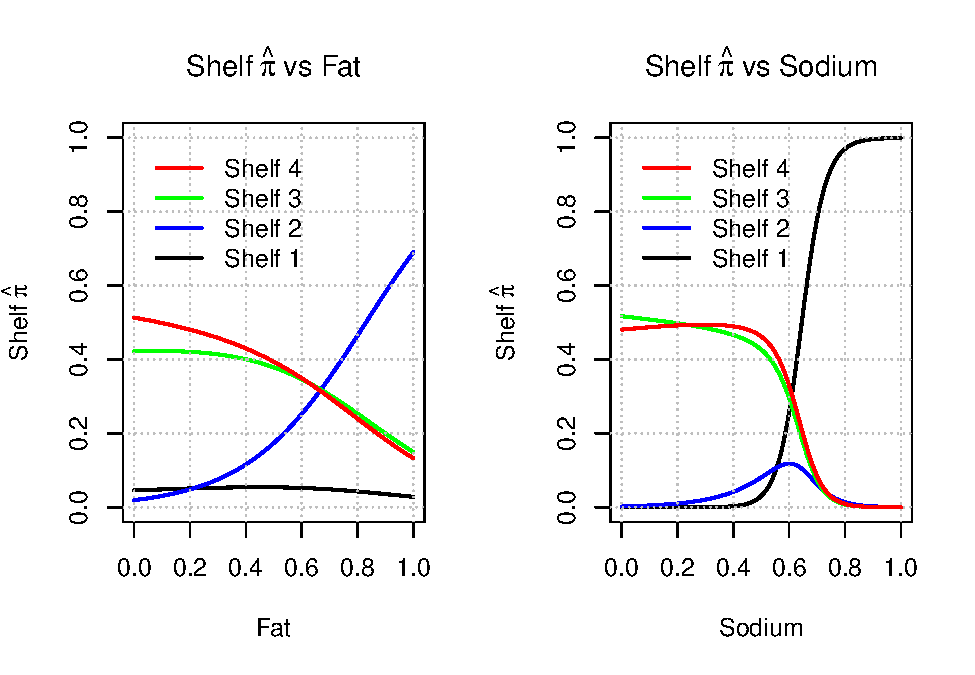
\includegraphics{HeatherFeinstein_DavidHarding_CharlotteSwavola.Rmd_files/figure-latex/unnamed-chunk-12-1.pdf}

\newpage

\begin{enumerate}
\def\labelenumi{\alph{enumi}.}
\setcounter{enumi}{7}
\tightlist
\item
  Estimate odds ratios and calculate corresponding confidence intervals
  for each explanatory variable. Relate your interpretations back to the
  plots constructed for this exercise.
\end{enumerate}

\begin{Shaded}
\begin{Highlighting}[]
\CommentTok{# Information about each variable to help with choosing c. Leave out Shelf column}
\NormalTok{sd.cereal2<-}\KeywordTok{apply}\NormalTok{(}\DataTypeTok{X =}\NormalTok{ cereal2[,}\OperatorTok{-}\KeywordTok{c}\NormalTok{(}\DecValTok{1}\NormalTok{)], }\DataTypeTok{MARGIN =} \DecValTok{2}\NormalTok{, }\DataTypeTok{FUN =}\NormalTok{ sd)}
\CommentTok{# sd.cereal2}

\CommentTok{#convert sd into (g/serving) units for interpretation. 0-1 are percentages of the overall range for g/serving}
\NormalTok{sd_convert<-}\ControlFlowTok{function}\NormalTok{(sd,df_column,}\DataTypeTok{df_serving=}\NormalTok{cereal}\OperatorTok{$}\NormalTok{size_g)\{}
\NormalTok{  var_range<-}\KeywordTok{max}\NormalTok{(df_column}\OperatorTok{/}\NormalTok{df_serving)}\OperatorTok{-}\KeywordTok{min}\NormalTok{(df_column}\OperatorTok{/}\NormalTok{df_serving)}
  \KeywordTok{return}\NormalTok{(sd}\OperatorTok{*}\NormalTok{var_range)}
\NormalTok{\}}


\NormalTok{c.value<-}\KeywordTok{c}\NormalTok{(}\DecValTok{1}\NormalTok{, sd.cereal2)  }\CommentTok{# class = 1 is first value}
\NormalTok{c.value<-c.value[}\DecValTok{2}\OperatorTok{:}\DecValTok{4}\NormalTok{] }\CommentTok{# drop intercept from c.value}
\KeywordTok{round}\NormalTok{(c.value,}\DecValTok{2}\NormalTok{)}
\end{Highlighting}
\end{Shaded}

\begin{verbatim}
##  sugar    fat sodium 
##   0.27   0.30   0.23
\end{verbatim}

\begin{Shaded}
\begin{Highlighting}[]
\NormalTok{units<-}\KeywordTok{c}\NormalTok{(}\DataTypeTok{g_serving=}\KeywordTok{sd_convert}\NormalTok{(c.value[}\DecValTok{1}\NormalTok{],cereal}\OperatorTok{$}\NormalTok{sugar_g),}\DataTypeTok{g_serving=}\KeywordTok{sd_convert}\NormalTok{(c.value[}\DecValTok{2}\NormalTok{],cereal}\OperatorTok{$}\NormalTok{fat_g),}\DataTypeTok{mg_serving=}\KeywordTok{sd_convert}\NormalTok{(c.value[}\DecValTok{3}\NormalTok{],cereal}\OperatorTok{$}\NormalTok{sodium_mg))}
\KeywordTok{round}\NormalTok{(units,}\DecValTok{2}\NormalTok{)}
\end{Highlighting}
\end{Shaded}

\begin{verbatim}
##   g_serving.sugar     g_serving.fat mg_serving.sodium 
##              0.15              0.03              2.46
\end{verbatim}

\begin{Shaded}
\begin{Highlighting}[]
\CommentTok{# beta.hat_jr for r = 1, 2, 3  and j = 2, 3, 4}
\NormalTok{beta.hat2<-}\KeywordTok{coefficients}\NormalTok{(mod.fit)[}\DecValTok{1}\NormalTok{,}\DecValTok{2}\OperatorTok{:}\DecValTok{4}\NormalTok{]}
\NormalTok{beta.hat3<-}\KeywordTok{coefficients}\NormalTok{(mod.fit)[}\DecValTok{2}\NormalTok{,}\DecValTok{2}\OperatorTok{:}\DecValTok{4}\NormalTok{]}
\NormalTok{beta.hat4<-}\KeywordTok{coefficients}\NormalTok{(mod.fit)[}\DecValTok{3}\NormalTok{,}\DecValTok{2}\OperatorTok{:}\DecValTok{4}\NormalTok{]}
\end{Highlighting}
\end{Shaded}

\begin{Shaded}
\begin{Highlighting}[]
\CommentTok{# Odds ratios for j = 2 vs. j = 1 }
\NormalTok{OR2_}\DecValTok{1}\NormalTok{<-}\KeywordTok{exp}\NormalTok{(c.value}\OperatorTok{*}\NormalTok{beta.hat2)}
\NormalTok{OR1_}\DecValTok{2}\NormalTok{<-}\DecValTok{1}\OperatorTok{/}\KeywordTok{exp}\NormalTok{(c.value}\OperatorTok{*}\NormalTok{beta.hat2)}

\CommentTok{# Odds ratios for j = 3 vs. j = 2 }
\NormalTok{OR3_}\DecValTok{2}\NormalTok{<-}\KeywordTok{exp}\NormalTok{(c.value}\OperatorTok{*}\NormalTok{beta.hat3)}
\NormalTok{OR2_}\DecValTok{3}\NormalTok{<-}\DecValTok{1}\OperatorTok{/}\KeywordTok{exp}\NormalTok{(c.value}\OperatorTok{*}\NormalTok{beta.hat3)}

\CommentTok{# for j = 3 vs j = 1}
\NormalTok{OR3_}\DecValTok{1}\NormalTok{<-OR3_}\DecValTok{2}\OperatorTok{*}\NormalTok{OR2_}\DecValTok{1}
\NormalTok{OR1_}\DecValTok{3}\NormalTok{<-}\DecValTok{1}\OperatorTok{/}\NormalTok{OR3_}\DecValTok{1}

\CommentTok{# Odds ratios for j = 4 vs. j = 3 }
\NormalTok{OR4_}\DecValTok{3}\NormalTok{<-}\KeywordTok{exp}\NormalTok{(c.value}\OperatorTok{*}\NormalTok{beta.hat4)}
\NormalTok{OR3_}\DecValTok{4}\NormalTok{<-}\DecValTok{1}\OperatorTok{/}\KeywordTok{exp}\NormalTok{(c.value}\OperatorTok{*}\NormalTok{beta.hat4)}

\CommentTok{# for j = 4 vs j = 1}
\NormalTok{OR4_}\DecValTok{1}\NormalTok{<-OR4_}\DecValTok{3}\OperatorTok{*}\NormalTok{OR3_}\DecValTok{1}
\NormalTok{OR1_}\DecValTok{4}\NormalTok{<-}\DecValTok{1}\OperatorTok{/}\NormalTok{OR4_}\DecValTok{1} 

\CommentTok{# for j = 4 vs j = 2}
\NormalTok{OR4_}\DecValTok{2}\NormalTok{<-OR4_}\DecValTok{3}\OperatorTok{*}\NormalTok{OR3_}\DecValTok{2}
\NormalTok{OR2_}\DecValTok{4}\NormalTok{<-}\DecValTok{1}\OperatorTok{/}\NormalTok{OR4_}\DecValTok{2}
\end{Highlighting}
\end{Shaded}

\begin{Shaded}
\begin{Highlighting}[]
\CommentTok{#build dataframes}
\NormalTok{OR_base=}\KeywordTok{data.frame}\NormalTok{(}\DataTypeTok{OR2_1=}\KeywordTok{round}\NormalTok{(OR2_}\DecValTok{1}\NormalTok{,}\DecValTok{2}\NormalTok{),}
                    \DataTypeTok{OR3_1=}\KeywordTok{round}\NormalTok{(OR3_}\DecValTok{1}\NormalTok{,}\DecValTok{2}\NormalTok{),}
                    \DataTypeTok{OR4_1=}\KeywordTok{round}\NormalTok{(OR4_}\DecValTok{1}\NormalTok{,}\DecValTok{2}\NormalTok{),}
                    \StringTok{"-"}\NormalTok{=}\KeywordTok{c}\NormalTok{(}\StringTok{"-"}\NormalTok{,}\StringTok{"-"}\NormalTok{,}\StringTok{"-"}\NormalTok{),}
                    \DataTypeTok{OR1_2=}\KeywordTok{round}\NormalTok{(OR1_}\DecValTok{2}\NormalTok{,}\DecValTok{2}\NormalTok{),}
                    \DataTypeTok{OR3_2=}\KeywordTok{round}\NormalTok{(OR3_}\DecValTok{2}\NormalTok{,}\DecValTok{2}\NormalTok{),}
                    \DataTypeTok{OR4_2=}\KeywordTok{round}\NormalTok{(OR4_}\DecValTok{2}\NormalTok{,}\DecValTok{2}\NormalTok{),}
                    \StringTok{"-"}\NormalTok{=}\KeywordTok{c}\NormalTok{(}\StringTok{"-"}\NormalTok{,}\StringTok{"-"}\NormalTok{,}\StringTok{"-"}\NormalTok{),}
                    \DataTypeTok{OR1_3=}\KeywordTok{round}\NormalTok{(OR1_}\DecValTok{3}\NormalTok{,}\DecValTok{2}\NormalTok{),}
                    \DataTypeTok{OR2_3=}\KeywordTok{round}\NormalTok{(OR2_}\DecValTok{3}\NormalTok{,}\DecValTok{2}\NormalTok{),}
                    \DataTypeTok{OR4_3=}\KeywordTok{round}\NormalTok{(OR4_}\DecValTok{3}\NormalTok{,}\DecValTok{2}\NormalTok{),}
                    \StringTok{"-"}\NormalTok{=}\KeywordTok{c}\NormalTok{(}\StringTok{"-"}\NormalTok{,}\StringTok{"-"}\NormalTok{,}\StringTok{"-"}\NormalTok{),}
                    \DataTypeTok{OR1_4=}\KeywordTok{round}\NormalTok{(OR1_}\DecValTok{4}\NormalTok{,}\DecValTok{2}\NormalTok{),}
                    \DataTypeTok{OR2_4=}\KeywordTok{round}\NormalTok{(OR2_}\DecValTok{4}\NormalTok{,}\DecValTok{2}\NormalTok{),}
                    \DataTypeTok{OR3_4=}\KeywordTok{round}\NormalTok{(OR3_}\DecValTok{4}\NormalTok{,}\DecValTok{2}\NormalTok{))}
\end{Highlighting}
\end{Shaded}

\begin{Shaded}
\begin{Highlighting}[]
\NormalTok{OR_base}
\end{Highlighting}
\end{Shaded}

\begin{verbatim}
##        OR2_1 OR3_1 OR4_1 X. OR1_2 OR3_2 OR4_2 X..1    OR1_3  OR2_3 OR4_3
## sugar   2.06  0.08   0.0  -  0.48  0.04  0.00    -    12.98  26.81  0.05
## fat     3.37  2.85   2.2  -  0.30  0.85  0.65    -     0.35   1.18  0.77
## sodium  0.02  0.00   0.0  - 55.74  0.00  0.00    - 17355.07 311.36  0.00
##        X..2      OR1_4    OR2_4  OR3_4
## sugar     -     278.95   575.96  21.48
## fat       -       0.45     1.53   1.30
## sodium    - 5038277.64 90390.00 290.31
\end{verbatim}

\begin{Shaded}
\begin{Highlighting}[]
\CommentTok{# Wald CIs}
\NormalTok{conf.beta<-}\KeywordTok{confint}\NormalTok{(}\DataTypeTok{object =}\NormalTok{ mod.fit, }\DataTypeTok{level =} \FloatTok{0.95}\NormalTok{)}
\CommentTok{# round(conf.beta,2)  # Results are stored in a 3D array}
\CommentTok{# conf.beta[2:4,1:2,1]  # C.I.s for beta_2r}
\CommentTok{# conf.beta[2:4,1:2,2]  # C.I.s for beta_3r}
\CommentTok{# conf.beta[2:4,1:2,3]  # C.I.s for beta_4r}
\CommentTok{#CI for probability based on variable entry}

\CommentTok{# CIs for OR}
\NormalTok{ci.OR2<-}\KeywordTok{exp}\NormalTok{(c.value}\OperatorTok{*}\NormalTok{conf.beta[}\DecValTok{2}\OperatorTok{:}\DecValTok{4}\NormalTok{,}\DecValTok{1}\OperatorTok{:}\DecValTok{2}\NormalTok{,}\DecValTok{1}\NormalTok{])}
\NormalTok{ci.OR3<-}\KeywordTok{exp}\NormalTok{(c.value}\OperatorTok{*}\NormalTok{conf.beta[}\DecValTok{2}\OperatorTok{:}\DecValTok{4}\NormalTok{,}\DecValTok{1}\OperatorTok{:}\DecValTok{2}\NormalTok{,}\DecValTok{2}\NormalTok{])  }
\NormalTok{ci.OR4<-}\KeywordTok{exp}\NormalTok{(c.value}\OperatorTok{*}\NormalTok{conf.beta[}\DecValTok{2}\OperatorTok{:}\DecValTok{4}\NormalTok{,}\DecValTok{1}\OperatorTok{:}\DecValTok{2}\NormalTok{,}\DecValTok{3}\NormalTok{]) }

\StringTok{"Shelf 2,3,4 vs Shelf 1"}
\end{Highlighting}
\end{Shaded}

\begin{verbatim}
## [1] "Shelf 2,3,4 vs Shelf 1"
\end{verbatim}

\begin{Shaded}
\begin{Highlighting}[]
\KeywordTok{round}\NormalTok{(}\KeywordTok{data.frame}\NormalTok{(}\DataTypeTok{low =}\NormalTok{ ci.OR2[,}\DecValTok{1}\NormalTok{], }\DataTypeTok{up =}\NormalTok{ ci.OR2[,}\DecValTok{2}\NormalTok{]), }\DecValTok{2}\NormalTok{) }\CommentTok{#RELATIVE TO SHELF 1}
\end{Highlighting}
\end{Shaded}

\begin{verbatim}
##         low    up
## sugar  0.14 29.68
## fat    0.87 13.04
## sodium 0.00  0.44
\end{verbatim}

\begin{Shaded}
\begin{Highlighting}[]
\KeywordTok{round}\NormalTok{(}\KeywordTok{data.frame}\NormalTok{(}\DataTypeTok{low =}\NormalTok{ ci.OR3[,}\DecValTok{1}\NormalTok{], }\DataTypeTok{up =}\NormalTok{ ci.OR3[,}\DecValTok{2}\NormalTok{]), }\DecValTok{2}\NormalTok{) }
\end{Highlighting}
\end{Shaded}

\begin{verbatim}
##         low   up
## sugar  0.00 0.49
## fat    0.21 3.49
## sodium 0.00 0.12
\end{verbatim}

\begin{Shaded}
\begin{Highlighting}[]
\KeywordTok{round}\NormalTok{(}\KeywordTok{data.frame}\NormalTok{(}\DataTypeTok{low =}\NormalTok{ ci.OR4[,}\DecValTok{1}\NormalTok{], }\DataTypeTok{up =}\NormalTok{ ci.OR4[,}\DecValTok{2}\NormalTok{]), }\DecValTok{2}\NormalTok{) }
\end{Highlighting}
\end{Shaded}

\begin{verbatim}
##         low   up
## sugar  0.00 0.61
## fat    0.19 3.16
## sodium 0.00 0.13
\end{verbatim}

\begin{Shaded}
\begin{Highlighting}[]
\StringTok{"Shelf 3 vs Shelf 2"}
\end{Highlighting}
\end{Shaded}

\begin{verbatim}
## [1] "Shelf 3 vs Shelf 2"
\end{verbatim}

\begin{Shaded}
\begin{Highlighting}[]
\KeywordTok{round}\NormalTok{(}\KeywordTok{data.frame}\NormalTok{(}\DataTypeTok{low =}\NormalTok{ ci.OR3[,}\DecValTok{1}\NormalTok{]}\OperatorTok{/}\NormalTok{ci.OR2[,}\DecValTok{1}\NormalTok{], }\DataTypeTok{up =}\NormalTok{ ci.OR3[,}\DecValTok{2}\NormalTok{]}\OperatorTok{/}\NormalTok{ci.OR2[,}\DecValTok{2}\NormalTok{]), }\DecValTok{2}\NormalTok{) }\CommentTok{#shelf 3 relative to 2}
\end{Highlighting}
\end{Shaded}

\begin{verbatim}
##         low   up
## sugar  0.02 0.02
## fat    0.24 0.27
## sodium 0.11 0.28
\end{verbatim}

\begin{Shaded}
\begin{Highlighting}[]
\StringTok{"Shelf 4 vs Shelf 3"}
\end{Highlighting}
\end{Shaded}

\begin{verbatim}
## [1] "Shelf 4 vs Shelf 3"
\end{verbatim}

\begin{Shaded}
\begin{Highlighting}[]
\KeywordTok{round}\NormalTok{(}\KeywordTok{data.frame}\NormalTok{(}\DataTypeTok{low =}\NormalTok{ ci.OR4[,}\DecValTok{1}\NormalTok{]}\OperatorTok{/}\NormalTok{ci.OR3[,}\DecValTok{1}\NormalTok{], }\DataTypeTok{up =}\NormalTok{ ci.OR4[,}\DecValTok{2}\NormalTok{]}\OperatorTok{/}\NormalTok{ci.OR3[,}\DecValTok{2}\NormalTok{]), }\DecValTok{2}\NormalTok{) }\CommentTok{#shelf 4 relative to 3}
\end{Highlighting}
\end{Shaded}

\begin{verbatim}
##         low   up
## sugar  1.26 1.24
## fat    0.92 0.91
## sodium 1.08 1.06
\end{verbatim}

\textbf{Odds ratio interpretations:} The \(c\) values (in
\(e^{c\beta_{jr}}\)) used to evaluate the odds ratios for each component
were calculated as 1 standard deviation unit. In grams per serving,
these \(c\) values are 0.15 g/serving of sugar, 0.03 g/serv fat, and
2.46 mg/serv sodium.

Evaluating sugar first, for each c-value increase in sugar, the odds
that the cereal would be on shelf 3 are 21.48 times as large as the odds
it would be on shelf 4, 12.98 times as large that it'd be on shelf 1 as
shelf 3, and 2.06 times as large that it would be on shelf 2 as shelf 1.
This matches the \(\hat{\pi}\) graph for sugar as shelves 1 and 2 have
the highest probabilities for increased sugar content, however doesn't
match the relatioship between 3 and 4. This discrepancy may be a result
of a smoothing error, as shelf 3 has an overall wider range of sugar
values, including some at higher sugar levels as the odds ratios
suggest, but also has more samples at lower sugar values than shelf 4.
Incorporating the confidence intervals, the CI of the odds ratio that
the cereal will appear on shelf 2 vs shelf 1 includes 1, so we cannot
definitively say the odds the cereal will be on shelf 2 are larger than
shelf 1. We can, however, say that the odds the cereal will be on
shelves 3 or 4 relative to shelf 1 are less than 1 for each unit
increase in sugar.

Looking at fat, again the odds that a cereal will be on shelf 2 are at
least twice as large as the odds of the other shelves. The \(\hat{\pi}\)
graphs echo this, for as the fat content increases, the likelihood the
cereal will appear 2 increases while all others decrease. Again, The
odds ratio confidence intervals span 1 for shelf 2 vs shelf 1, however
are entirely below 1 for shelf 3 vs shelf 2 and shelf 4 vs shelf 3,
indicating that the odds of the cereal to be on shelf 2 are larger than
shelf 3 or 4 for an increase in fat.

Now, the odds ratios for sodium reach extreme numbers, especially
relative to shelf 1. The behavior of the \(/hat{/pi}\) vs sodium content
for shelf 1 increases from 0 to 1 in about 0.3 units, almost the same as
our c-value, potentially because only high-sodium samples appear on
shelf 1. This is reiterated by the confidence intervals, as all the
other shelf intervals are below 0.5 relative to shelf 1. This means that
for each unit increase in sodium, the odds that a cereal appears on any
other shelf are at most 1/2 as large as the odds that the cereal appears
on shelf 1.


\end{document}
